\section{Methodologies explored}
We explore recent literature related to definition modeling and present our findings related to explored methodology in this section. Definition generation is a critical task where multiple definitions can be generated for a single target word. Therefore, researchers focus on improving the definition generation task by applying various techniques. Two key technical aspects are observed in the literature: definition generation and word embedding. Definition generation is considered a language modeling task, where we predict the joint probability of a  sequence of words, and based on maximum likelihood, the highest probability sequence is returned as a definition of a given target word. Since the output definition mostly depends on the context of the target word, vector representation of such target words is essential to capture context scenarios. Below we discuss both of these aspects, language modeling, and word embedding
techniques and related literature.

\subsection{Language models and definition generation}
A definition model is a language model that is trained on a set of definitions
\cite{noraset_definition_2016}. The goal of a definition model is to learn to
generate a definition for a given term. The probability of generating the $t$-th
word in a definition depends on the previous words in the definition and
the word to be defined in Eq \ref{eq:definition_model}.

\begin{equation}
    \label{eq:definition_model}
    p(\textbf{d} | w) = \prod_{t=1}^{T} p(d_t | d_1,...,d_{t-1}, w)
\end{equation}

\noindent
where \textbf{d} is the generated definition as a vector of words ($\textbf{d} =
    [d_1, ..., d_T]$) and $w$ is the word or phrase to be defined.

Noraset et al.~\cite{noraset_definition_2016} condition a \textit{recurrent neural network} (RNN) to generate a definition from an input seed word. They modify the model by updating the output of the recurrent unit with an update
function inspired by \textit{gated recurrent unit} (GRU) update gate~\cite{noraset_definition_2016}. They apply pretrained word embeddings generated from \textit{Word2Vec} \cite{mikolov_efficient_2013}. In later
work, it was shown that the definition model does not generate definitions for words with ambiguous word sense, especially polysemantic words \cite{gadetsky_conditional_2018}. The following context-aware definition model was proposed by Gadetsky et al. \cite{gadetsky_conditional_2018} to tackle this challenge. To generate a definition, authors
use an attention-based skip-gram model to extract dimensions from the embedding which contain the most relevant information \cite{gadetsky_conditional_2018}. They extend Eq \ref{eq:definition_model} by adding a context term which is a contextual phrase or example sentence to be used in the generation of the definition as defined in Eq \ref{eq:context_aware_definition_model}.

\begin{equation}
    \label{eq:context_aware_definition_model}
    p(\textbf{d} | w, \textbf{c}) = \prod_{t=1}^{T} p(d_t | d_1,...,d_{t-1}, w, \textbf{c})
\end{equation}

\noindent
where \textbf{c} is the context phrase ($\textbf{c} = [c_1, ..., c_T]$).

Researchers apply \textit{sequence-to-sequence} algorithms and represented
definitions vectors by formulating language modeling to capture sequence
features and context \cite{bevilacqua_generationary_2020, huang_cdm_2021,
    kabiri_evaluating_2020, washio_bridging_2019, reid_vcdm_2020}. Among these
algorithms, RNN and \textit{long-short-term-memory network} (LSTM) are important
as they can capture semantic information across words in a sentence as
sequential data. Not all words are equally important in a definition as they
have different contributions in the definition generations. Transformer-based
techniques help focus on the contribution of particular words in the definition.
Therefore, few researchers also focus on transformer networks such as
\textit{bidirectional encoder representations from transformers} (BERT) and
denoising decoder \cite{devlin2018bert, lewis2019bart}.

The definition usually contains summarized information about the given target word. Huang et al.~\cite{huang_cdm_2021} focus on generating definition by using extracted self- and correlative definition information of a given term from the
web. The authors in~\cite{huang_cdm_2021} extracted sentences containing the target term and then ranked
sentences using deployed BERT-based model and extracted self-definitional information (SDI) from Wikipedia. Then, they design a conditional sequence-to-sequence model, denoising decoder, and fine-tune parameter with extracted information and general definition for a given term.

Definition modeling works similarly to language models to generate definition sentences and corresponding probabilities. Gadetsky et al.~\cite{gadetsky_conditional_2018} proposed a \textit{conditional RNN} based
language model for developing the definition of a given word. First, they created AdaGram based RNN model and conditioned it on adaptive skip-gram vector representation. Their second model focused on an attention-based skip-gram to generate a definition for a corresponding context.

Li et al. \cite{li_explicit_2020} proposed \textit{explicit semantic decomposition} (ESD) to decompose the meaning of the word into semantic components and model them with the discrete latent variable for definition generation. This model comprises an \textit{encoder}, \textit{decoder}, and
\textit{semantic component predictor}. The encoder consists of two components: word encoder and \textit{bidirectional LSTM} (Bi-LSTM) context encoder. Word encoder creates low-dimensional vectors of the word, whereas
the Bi-LSTM context encoder incorporates context information. Semantic component predictor model approximate posterior using Bi-LSTM model.
Finally, LSTM based definition decoder generates a definition from the encoded data.

Bevilacqua et al. \cite{bevilacqua_generationary_2020} propose a span-based
encoding model that is used to map occurrences of target words or phrases in a
given context and generate a gloss. Using the probability of a gloss for a given
context-word pair, their method can perform classification by selecting the
gloss with the highest probability. The textual gloss is then applied to define
the context and word.

Ishiwatari et al. \cite{ishiwatari_learning_2019} solve the problem of unknown
phrase definition by incorporating local and global context information while
defining a word. Local context refers to the sequence of neighboring words of
the target word. In contrast, the global context refers to the entire document
or even searching the web text to find other occurrences of the expression to
understand the meaning. The authors in \cite{ishiwatari_learning_2019} proposed LSTM based encoder-decoder model where a gated unit deployed reduces the ambiguity of local and global context.

Mickus et al. \cite{mickus_mark_2019} argue that due to the \textit{distribution
    hypothesis} (words with similar distribution have similar meaning), the
problem of definition modeling should be reformulated as a
sequence-to-sequence task, where the input sequence is a sentence with the
word to be defined highlighted \cite{mickus_mark_2019}. The input sequence
provides the context necessary to generate the output definition. Zhu et al.
\cite{zhu_multi_2019} study the multi-sense definition modeling task using
the Gumble-softmax approach. This approach decomposes word senses from the
pre-trained word embeddings and applies LSTM sequence-to-sequence modeling
to generate definition sentences.

Reid et al. \cite{reid_vcdm_2020} introduced a variational generative model to
produce a definition that directly combines lexical and distributional semantics
using the continuous latent variable. Initially, the BERT model is fine-tuned
with phrase-context pairs, and in the context, sentence lexeme form is used to
reduce the differences in the word or phrase. Once the BERT model encodes the
definition, the proposed approach applies a neural definition inference module
to compute approximate posterior from the variational distribution of the
definition. During definition generation, that is, sequence of word generation
task, this model deploys LSTM enabled variational contextual definition modeler
to generate a sequence of words as the definition.

Chang et al. \cite{chang_what_2019} explore contextualized embedding for
definition modeling - to get contextualized word embedding the authors used the
pretrained \textit{embeddings from language models} (ELMo) and BERT model. The authors in \cite{chang_what_2019} reformulate the problem of
definition modeling from text generation to text classification. Instead of
mapping the classifier with discrete labels, all ground truth
definitions are encoded in the embedding space via learning a mapping function. Then, they generate an embedding for a given
word-in-context and apply k-nearest neighbor to predict multiple
definitions for a given target word from a corpus of existing definition
embeddings. Their results show state-of-the-art performance on the task of
definition modeling.

% non-english
\noindent\textbf{Non-English languages:}
Most definition modeling methods focus on generating definitions in English for English words. Definition generation was also explored in the non-English language. Since the definition depends on the lexical properties, language
syntax, and phrase construction, different languages influence the proposed methodology to capture the definition of a specific word. For example, in parataxis languages (e.g., Chinese), the meaning of a word is based on formation components (morphemes) combined by the formation rule (morphemes are combined to form words).

Zheng et al. \cite{zheng_decompose_2021} utilizes this word meaning formation
process in consideration to build a definition generation model where words
decompose into formation features and then use gating techniques to generate
definition. In this work, the authors in \cite{zheng_decompose_2021} develop morpheme features using the Bi-LSTM model and concatenate character-level embedding and pre-trained word embedding together. Finally, gated attention-based morpheme features with
attention-based context vector to form a feature vector. The definition generator employs a gated LSTM model that generates the definition using the feature vector.

Ni et al. \cite{ni_learning_2017} automatically generates explanations for
non-standard English expressions using sequence to sequence models. The authors
use two encoder approaches: a word-level LSTM-encoder encodes context information, and a character-level encoder encodes target non-standard terms
\cite{ni_learning_2017}. Kong et al. \cite{kong_toward_2020} fine-tune multilingual BERT and cross-lingual model and provide target word and examples sentence as context
to produce definition as output. This model can generate definitions in English
from various languages (e.g., Chinese to English).

Kabiri et al. \cite{kabiri_evaluating_2020} proposed context-agnostic
multi-sense definition generation model. The proposed RNN based model generates
multiple definitions based on a given target word type (polysemous word) and
incorporates the char-CNN model to capture affixes information. They associate
sense vectors with definitions and create a definition-to-sense and
sense-to-definition model. These definition models represented definition by
taking the average of the word embeddings of all the words. Their multi-sense
model demonstrates the ability to generate multi-sense embeddings across nine
languages from various language families.

\subsection{Word embedding}

\begin{figure}[h]
    \centering
    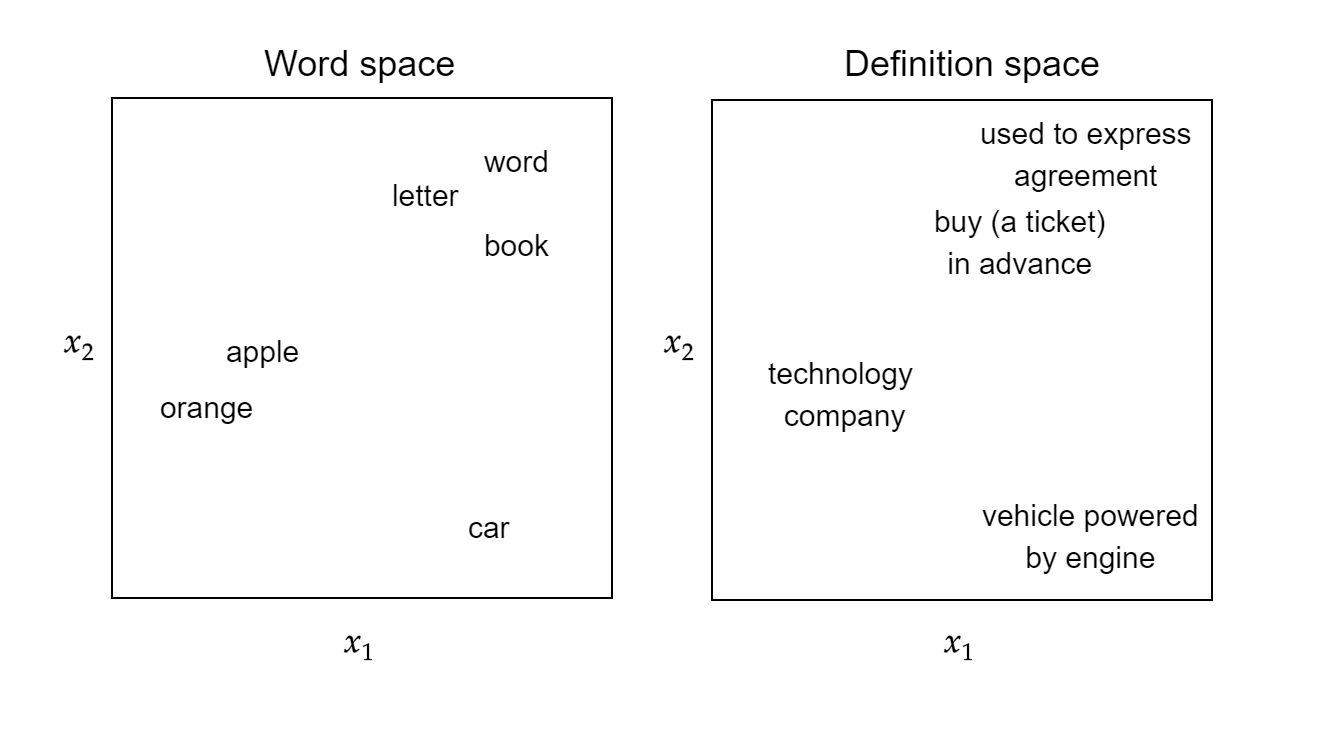
\includegraphics[width=0.8\textwidth]{assets/figures/embedding_space.png}
    \caption{An example of two vector spaces: word space and definition space. As vector representations, semantically similar
    words and definitions are closer together. Although word embedding vectors 
    can be quite large in practice, we represent them with two attributes for simplicity.}
    \label{fig:embedding_space}
\end{figure}

We can transform text or words into vector representations to analyze words effectively.  Figure \ref{fig:embedding_space} represents word space (2-D) by attaching several numerical
attributes to the words ($x_1$ and $x_2$). Word embeddings are fixed-length vectors representing words in a vector space such that similar words meanings have similar vector space representations. In  Word2Vec, a popular word embedding model, surrounding words are predicted from a given target word \cite{mikolov_efficient_2013}. For an example, we will use the sentence \textit{the height of Mount Everest is 29029 feet}. Given a target word \textit{Mount}, we apply a context window of $\pm3$. The model will attempt to predict the three words preceding the target word (\textit{the height of}). The model will also attempt to predict the three words succeeding the target word (\textit{Everest is 29029}). In the prediction process, the model simultaneously learns the vector representation of words and maximizes the prediction
probability of the context window words.

The vector space representation is useful to measure the distance between words and do vector space calculations \cite{mikolov_distributed_2013}. In definition
modeling, the definition is also represented in a
vector space so that the candidate definition of a target word can easily be found from the vector space. An example is
shown in Figure \ref{fig:embedding_space}, where each definition is represented using two attributes: $x_1$ and $x_2$. In the definition modeling problem, word
to vector representation is key in modeling definitions for a given
term.

Bosc et al. \cite{bosc_auto_2018} exploited dictionary recursivity into
consideration and proposed an autoencoder-based word embedding algorithm, and
generated a single embedding per word—the proposed auto-encoder model comprises
of an LSTM encoder and decoder. The authors in \cite{bosc_auto_2018} introduced three embeddings:
definition embeddings produced by the proposed definition encoder, input
embeddings for the encoder, and output embeddings. While
modeling these embedding models, A consistency penalty is applied as
soft weight in their cost function to enforce input embedding and definition
embedding closer \cite{bosc_auto_2018}.

Washio et al. \cite{washio_bridging_2019}, the authors consider lexical-semantic
relations between the defined word and defining words using unsupervised methods
to propose definition modeling. To learn word embeddings, the authors proposed
LSTM-based encoder and decoder with an additional cost function to learn
word-pair embeddings in the decoder and capture lexical-semantic relations.
Dictionary embeddings often follow a genus and differentia structure for a
dictionary definition. Noraset et al.~\cite{noraset_definition_2016} capture
hypernyms embedding following proper genus database WebIsA containing hypernym
relations. In addition, the authors in \cite{noraset_definition_2016} incorporate char-CNN to capture affixes to
model gated-RNN based definition modeling.

Word embeddings are learned from large corpora. Therefore, it may consist of
biases such as gender, race, and religion. On the other hand, word dictionaries
contain unbiased, concise definitions. To overcome these biases by utilizing
pre-trained word-embedding, Kaneko et al. \cite{kaneko_dictionary_2021} apply
learned embedding from existing input word embeddings using encoder-decoder
architecture by defining a decoder cost function that considers dictionary
agreement as a constraint and decodes the debiased embedding.

Zhang et al. \cite{zhang_improving_2020} propose a novel framework by
formulating definition modeling and word-embedding as multitask learning
problems. The authors in \cite{zhang_improving_2020} presented two types of multitasking models to combine
usage and definition modeling. First, the authors in \cite{zhang_improving_2020} used the GRU-based context
encoder model as a semantic generative network to generate word embedding. This
approach encodes context sequences into continuous vectors and generates a
fixed-size sentence embedding. After that, self-attention is applied to consider
the target word sense. Then, this model learns context-sensitive word embedding by
fine-tuning ELMo models. Finally, the authors in \cite{zhang_improving_2020} formulated multitask sequence-to-sequence modeling for usage modeling to generate definition and example sentences.

\subsection{Evaluation criteria}

A variety of evaluation criteria are used to evaluate generated definitions.
Table \ref{tab:eval} lists the evaluation criteria used in the definition
modeling task. The evaluation takes the reference and candidate definitions as input and outputs a score on how well the candidate matches the reference. The reference definition is
the correct definition of the source word or phrase, typically provided by a
dictionary. The candidate definition is the machine-generated definition. We
provide brief descriptions of the evaluation criteria used.

\begin{table}[h]
    \centering
    \caption{Evaluation criteria used in definition modeling.}
    \begin{tabular}{|ll|}
        \hline
        Criteria          & Methods
        \\
        \hline
        BLEU              & \cite{bevilacqua_generationary_2020,
            gadetsky_conditional_2018, huang_cdm_2021, ishiwatari_learning_2019,
            kabiri_evaluating_2020, li_explicit_2020, noraset_definition_2016,
            reid_vcdm_2020, washio_bridging_2019}                                \\
        Perplexity        & \cite{bevilacqua_generationary_2020,
            gadetsky_conditional_2018, mickus_mark_2019,
            noraset_definition_2016, washio_bridging_2019}                       \\
        ROUGE-L           & \cite{bevilacqua_generationary_2020,
            chang_what_2019, huang_cdm_2021}                                     \\
        METEOR            & \cite{bevilacqua_generationary_2020, huang_cdm_2021,
            li_explicit_2020}                                                    \\
        BERTScore         & \cite{bevilacqua_generationary_2020, huang_cdm_2021,
            reid_vcdm_2020}
        \\
        Human             & \cite{ishiwatari_learning_2019, li_explicit_2020,
            reid_vcdm_2020}
        \\
        Precision         & \cite{chang_what_2019}
        \\
        Cosine similarity & \cite{chang_what_2019}
        \\
        \hline
    \end{tabular}
    \label{tab:eval}
\end{table}


\noindent\textbf{BLEU}: \textit{Bilingual evaluation understudy} (BLEU) is a standard algorithm used to evaluate machine translations~\cite{papineni_2002_bleu}. BLEU score is calculated as n-gram precision, or the ratio of correct n-grams to the total number of output n-grams. A drawback of the BLEU score is that it matches correct n-grams and thus may not give a good score to an acceptable generated
definition.

\noindent\textbf{Perplexity}: \textit{Perplexity} is related to entropy, which is a
measurement of the uncertainty of a probability distribution and is normalized
by sentence length. The perplexity is a measure of the difficulty of generating
a sentence. The lower the perplexity, the more natural the sentence is for the
model.

\noindent\textbf{ROUGE-L}: \textit{Recall-oriented understudy for gisting evaluation}
(ROUGE) measures the matching n-grams between the reference and candidate
definitions \cite{lin_2004_rouge}. ROUGE-L is a modified version of ROUGE that
uses the \textit{longest common subsequence} to measure the similarity between
the two definitions. An advantage of ROUGE-L is that it automatically determines
the longest in-sequence common n-grams.

\noindent\textbf{METEOR}: \textit{Metric for evaluation of translation with explicit
    ordering} (METEOR) is a metric that is based on unigram matching between the
reference and candidate translations \cite{banerjee_2005_meteor}. It
computes a score based on the harmonic mean of precision and recall.

\noindent\textbf{BERTScore}: \textit{Bidirectional encoder representations from
    transformers} (BERTScore) is a metric that computes a similarity score of
the candidate and reference definitions based on the pre-trained contextual
embeddings from BERT \cite{zhang_bertscore_2020}. In addition, BERTScore
computes precision, recall, and F1 measure.

\noindent\textbf{Cosine similarity}: \textit{Cosine similarity} is a measure of the
similarity between two vectors. It is simply calculated as the dot product of
the two vectors divided by the product of their magnitudes.

\noindent\textbf{Precision}: \textit{Precision} is a measure of the proportion of
correctly identified words in a sentence.

In principle, any other string similarity measure could be applied for this task~\cite{gali_2019_framework}. Human-based evaluation scores would be ideal due to
expert linguistic knowledge. However, in practice, collecting expert evaluation
is costly. As BERTScore takes advantage of semantic information, it correlates
better with human judgments and may be most useful for evaluating generated
definitions \cite{zhang_bertscore_2020}.

% make conclusion about which evaluation is most appropriate